% arara: xelatex: { shell: yes }
% arara: xelatex: { shell: yes }

\documentclass[czech,aspectratio=169]{beamer}

\usepackage{polyglossia}
\setmainlanguage{czech}

\usetheme{Madrid}
\usecolortheme{whale}

\useinnertheme{rectangles} %možnosti: default circles rectangles rounded inmargin
\useoutertheme{default} %možnosti: default, miniframes, smoothbars, sidebar, split, shadow, tree, smoothtree, infolines

\definecolor{CVUT}{HTML}{0065BD}
\setbeamercolor{structure}{bg=white,fg=CVUT}

% jako font prezentace nadefinujeme oficiální ČVUT písmo Technika
% https://www.cvut.cz/logo-a-graficky-manual  -- inforek, příhlášení přes celoškolské heslo
\usepackage{fontspec}
\setsansfont{Technika-Book}

\usepackage[style=iso-numeric]{biblatex}
\addbibresource{bybliography.bib} 

% vypneme navigační panel beamer (pro zapnutí zakomentujeme)
\beamertemplatenavigationsymbolsempty

% vygenerujeme slajdy s poznámkami
% \setbeameroption{show notes} 

% vygeneruje slajdy s poznámky vhodné pro promítání na dvou monitorech
% \usepackage{pgfpages}
% \setbeameroption{show notes on second screen}

% další balíčky
\usepackage{graphicx}
\usepackage{minted}
\usepackage{hyperref}
\usepackage{tikz}
\usepackage{pgfplots}
\usetikzlibrary{chains,fit,shapes}

% Údaje o prezentaci
\title[Webová aplikace pro výuku hry na ukulele]{Specializovaná webová aplikace pro výuku hry na ukulele}
\subtitle{Bakalářská práce}
\institute[FIT ČVUT v~Praze]{Fakulta informačních technologií \\ České vysoké učení technické v~Praze}
\author[D. Balarin]{Dan Balarin \\ Vedoucí práce: Ing. Marek Suchánek}
\date{24. 6. 2020}
\titlegraphic{
\includegraphics[width=.3\textwidth]{assets/logo-FIT}}


\begin{document}
\begin{frame}
    \titlepage
    \note{Nezapomenout pozdravit}
\end{frame}

% \begin{frame}
%     \tableofcontents
% \end{frame}

\section{Motivace}
\begin{frame}{Motivace}
    \begin{center}
        Vlastní výuka hry na ukulele
        \vskip5mm
        Aplikace s~nedostatečnou funkcionalitou
    \end{center}
    \note{Aplikace měli vždy částečnou funkcionalitu, ale ne spojenou v~jeden celek.}
    \note{Příkladem můžou být stránky s~texty a akordy písní bez metronomu nebo strumming patternu.}
\end{frame}

\section{Cíle}
\begin{frame}{Cíle}
    \begin{center}
        Hlavním cílem bylo \textbf{vytvoření webové aplikace} \\
        se zaměřením na \textbf{uživatelskou přívětivost}\\
        \textbf{pro začátečníky}.
        \vskip5mm
        Dílčím cílem bylo umožnit již \textbf{zkušenému}\\
        \textbf{hráči} vyhledat \textbf{akordy a text k písni}.
    \end{center}
\end{frame}

\section{Architektura aplikace}
\begin{frame}{Architektura aplikace}{Moduly}
    \begin{center}
        uls@\color{blue}<doména>\color{black}-\color{red}<react|nodejs|common>\color{black}
        \note{Domény jsou core, look, auth, user, ukulele}
        \\
        \pause
        uls@\color{red}<react|nodejs>\color{black}-package
    \end{center}
\end{frame}


\section{Implementace}
\begin{frame}{Implementace}
    \note{Zmínit NRG stack, Node, React GraphQL}
    \begin{itemize}
        \item TypeScript
        \item Jest
        \item Backend
              \begin{itemize}
                  \item Express.js
                  \item MongoDB
                  \item Apollo Server
              \end{itemize}
        \item Frontend
              \begin{itemize}
                  \item Express.js
                  \item React
                  \item Apollo Client
              \end{itemize}
    \end{itemize}
\end{frame}

\section{Architektura aplikace}
\begin{frame}{Architektura aplikace}{Clean Architecture}
    \begin{figure}
        \centering
        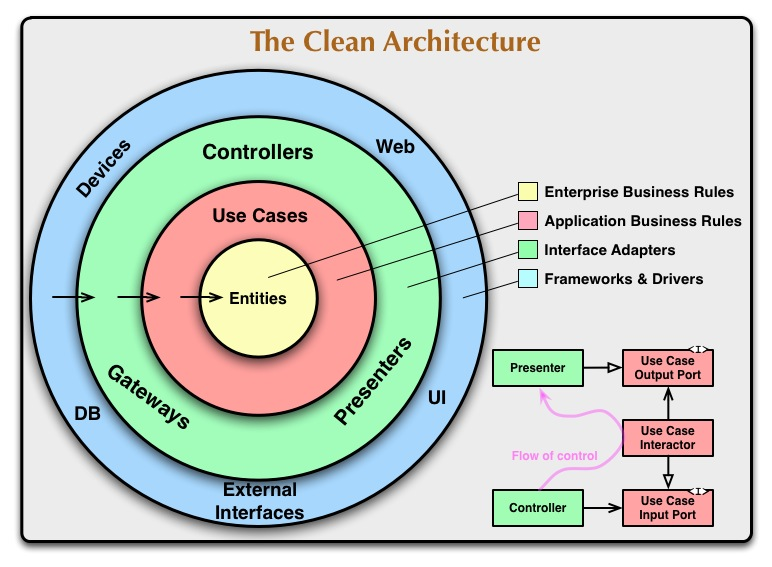
\includegraphics[width=.5\textwidth]{assets/clean_architecture.jpg}
        \caption{Clean Architecture [1]}
        \label{fig:clean_architecture}
    \end{figure}
\end{frame}

\section{Ukázka výsledné aplikace}
\begin{frame}{Ukázka výsledné aplikace}
    \begin{figure}
        \centering
        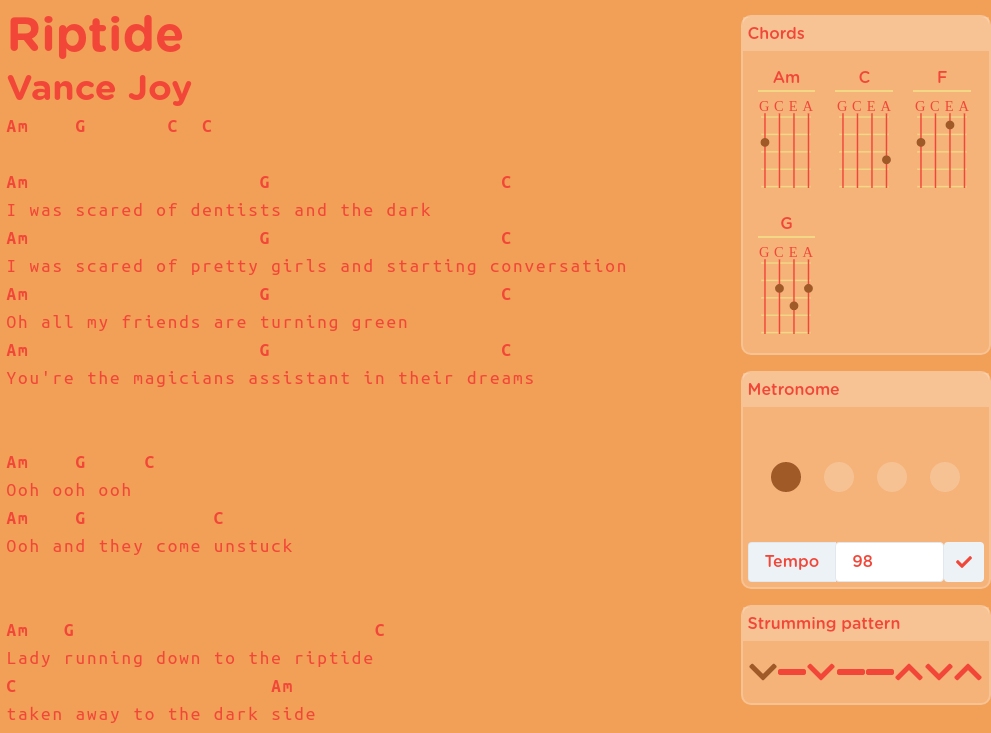
\includegraphics[width=.6\textwidth]{assets/screen.png}
    \end{figure}
\end{frame}

\section{Nasazování}
\begin{frame}{Nasazování}
    \centering
    \begin{tikzpicture}
        \tikzstyle{every path}=[very thick]
        \tikzstyle{cloud} = [draw, ellipse,fill=gray!20,minimum height=2em]
        \node[cloud](gha){GitHub Actions};
        \node[cloud](trigger)[above=of gha]{trigger};
        \node[cloud](deploy)[below=of gha]{Nasazení na VPS};
        \node[cloud](dockerhub)[left=of deploy]{Docker Hub};
        \node[cloud](smoke)[right=of deploy]{Smoke test};
        \draw[->] (trigger.south) -- (gha.north);
        \draw[->] (gha.south) to[out=-135,in=45] (dockerhub.15);
        \draw[->] (gha.south) -- (deploy.north);
        \draw[->] (gha.south) to[out=-45,in=135] (smoke.155);
    \end{tikzpicture}
\end{frame}

\begin{frame}{Shrnutí}
    \begin{itemize}
        \item provedena analýza trhu
        \item vytvořena funkční specifikace
        \item vytvořen lehce rozšiřitelný a udržovatelný prototyp
        \item otestováno unit testy
        \item vytvořena dokumentace
        \item automatické nasazování
    \end{itemize}
    \bigskip
    \begin{itemize}
        \item aplikace: \underline{http://shorturl.at/beoW6}
        \item dokumentace: \underline{http://shorturl.at/vDEZ7}
    \end{itemize}
\end{frame}

% \begin{frame}{Děkuji za pozornost}
%     \centering
%     Prostor na dotazy
% \end{frame}

\begin{frame}[noframenumbering]{Otázky oponenta}
    Otázka první: Proč?

    \vfill

    Odpověď: Prostě proto.
\end{frame}

\begin{frame}[noframenumbering]{Otázky oponenta}
    Otázka druhá: Proč?

    \vfill

    Odpověď: Prostě proto.
\end{frame}

\begin{frame}{Zdroje}
    \begin{itemize}
        \item [1] MARTIN, Robert Cecil. \emph{The Clean Architecture} [online]. 2012 [cit. 2020-05-25]. Dostupné z: \url{https://blog.cleancoder.com/uncle-bob/2012/08/13/the-clean-architecture.html}.
    \end{itemize}
\end{frame}


\end{document}
